
\section{VAM Beam--Swirl Interaction Spectrum}

\section*{1. Introduction}
In the Vortex Æther Model (VAM), fusion events are governed by the overlap between external beam-induced swirl modes and the natural swirl eigenfrequencies of vortex knots. This document formalizes the interaction and presents a spectral yield curve.

\textbf{What this adds to VAM:} This framework:
\begin{itemize}
\item Establishes a frequency-resolved mechanism for fusion driven by swirl-vortex coupling.
\item Enables prediction of yield via spectral overlap instead of thermal rates.
\item Introduces beam bandwidth and spectral shape as controllable fusion variables.
\item Allows engineering of resonance-based LENR experiments using gamma or ion beams.
\item Bridges vortex eigenmodes with experimental phenomena such as discrete nuclear activation thresholds.
\end{itemize}

\section*{2. Swirl Coupling Formalism}
We define the fusion excitation yield $Y_{\mathrm{VAM}}$ as the spectral overlap:
\begin{equation}
Y_{\mathrm{VAM}} = \int_0^\infty \rho_{\mathrm{beam}}(\omega) \cdot \sigma_{\mathrm{knot}}(\omega) , d\omega
\end{equation}

\noindent where:
\begin{itemize}
\item $\rho_{\mathrm{beam}}(\omega)$ is the Gaussian spectral energy density of the injected beam:

$\rho_{\mathrm{beam}}(\omega) = A \exp\left(-\frac{(\omega - \omega_0)^2}{2 \Delta \omega^2} \right)$
\item $\sigma_{\mathrm{knot}}(\omega)$ is the vortex knot's absorption spectrum modeled as a sum of Lorentzians:
$\sigma_{\mathrm{knot}}(\omega) = \sum_n \frac{B_n \Gamma_n^2}{(\omega - \omega_n)^2 + \Gamma_n^2}$
\end{itemize}

\section*{3. Numerical Simulation}
We model:
\begin{itemize}
\item A beam centered at frequency $\omega_0 = \frac{C_e}{r_c}$
\item Three vortex species with resonances near $\omega_0$
\end{itemize}

\begin{figure}[h!]
\centering
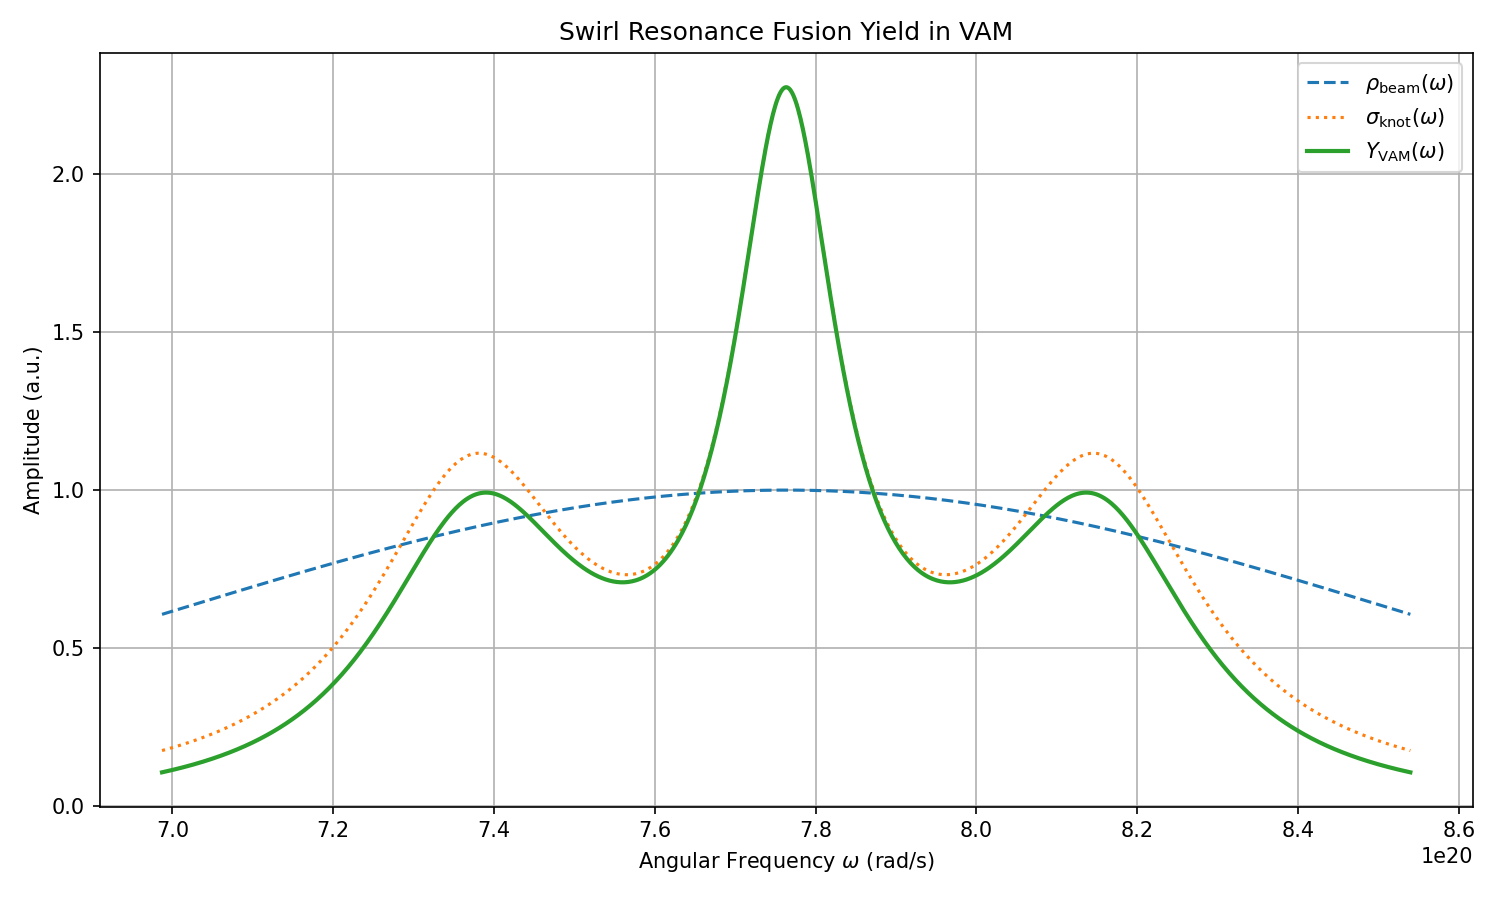
\includegraphics[width=0.9\textwidth]{../images/Appendix_BeamSwirlInteractionSpectrumImage2}
\caption{Spectral overlap of the injected beam (dashed), knot absorption spectrum (dotted), and resulting fusion yield $Y_{\mathrm{VAM}}(\omega)$ (solid). Resonant enhancement occurs where matching is maximal.}
\end{figure}

\section*{4. Interpretation}
The model confirms that fusion is enhanced when the injected swirl field (from laser-accelerated ions or gamma beams) matches one or more knot resonance modes. Broader beams engage multiple knot species; narrow-band beams offer precision tuning for maximal yield.

\textbf{Experimental relevance:} Discrete activation thresholds observed in gamma-induced fusion reactions \cite{Goryachev2020, Liu2022} support the prediction that nuclear systems respond preferentially to matched-frequency external fields. This spectral sensitivity aligns with VAM's core hypothesis of swirl–vortex resonance.
\section*{5. Time-Domain Interpretation: Pulse-Swirl Coupling}
In the time domain, the injected beam can be treated as a finite-duration pulse:
\begin{equation}
F(t) = , \text{Re} \left{ E_0 e^{-t^2/\tau^2} e^{i \omega_0 t} \right}
\end{equation}
The corresponding excitation in the knot is given by convolution with the knot\rqs s response function:
\begin{equation}
S(t) = \int_0^t F(t') K(t - t') , dt'
\end{equation}
Where $K(t)$ is the inverse Fourier transform of $\sigma_{\mathrm{knot}}(\omega)$. This formalism shows:
\begin{itemize}
\item Short pulses excite a wide range of knot modes (broadband excitation).
\item Long pulses selectively enhance specific resonant vortex eigenmodes.
\item The coherence time $\tau$ determines whether the excitation remains in phase with the vortex swirl.
\end{itemize}
The time-domain representation bridges real beam shaping strategies (e.g., Gaussian laser pulses) with knot activation dynamics and supports experimental tuning of pulse duration to control vortex coupling.
\begin{figure}[h!]
  \centering
  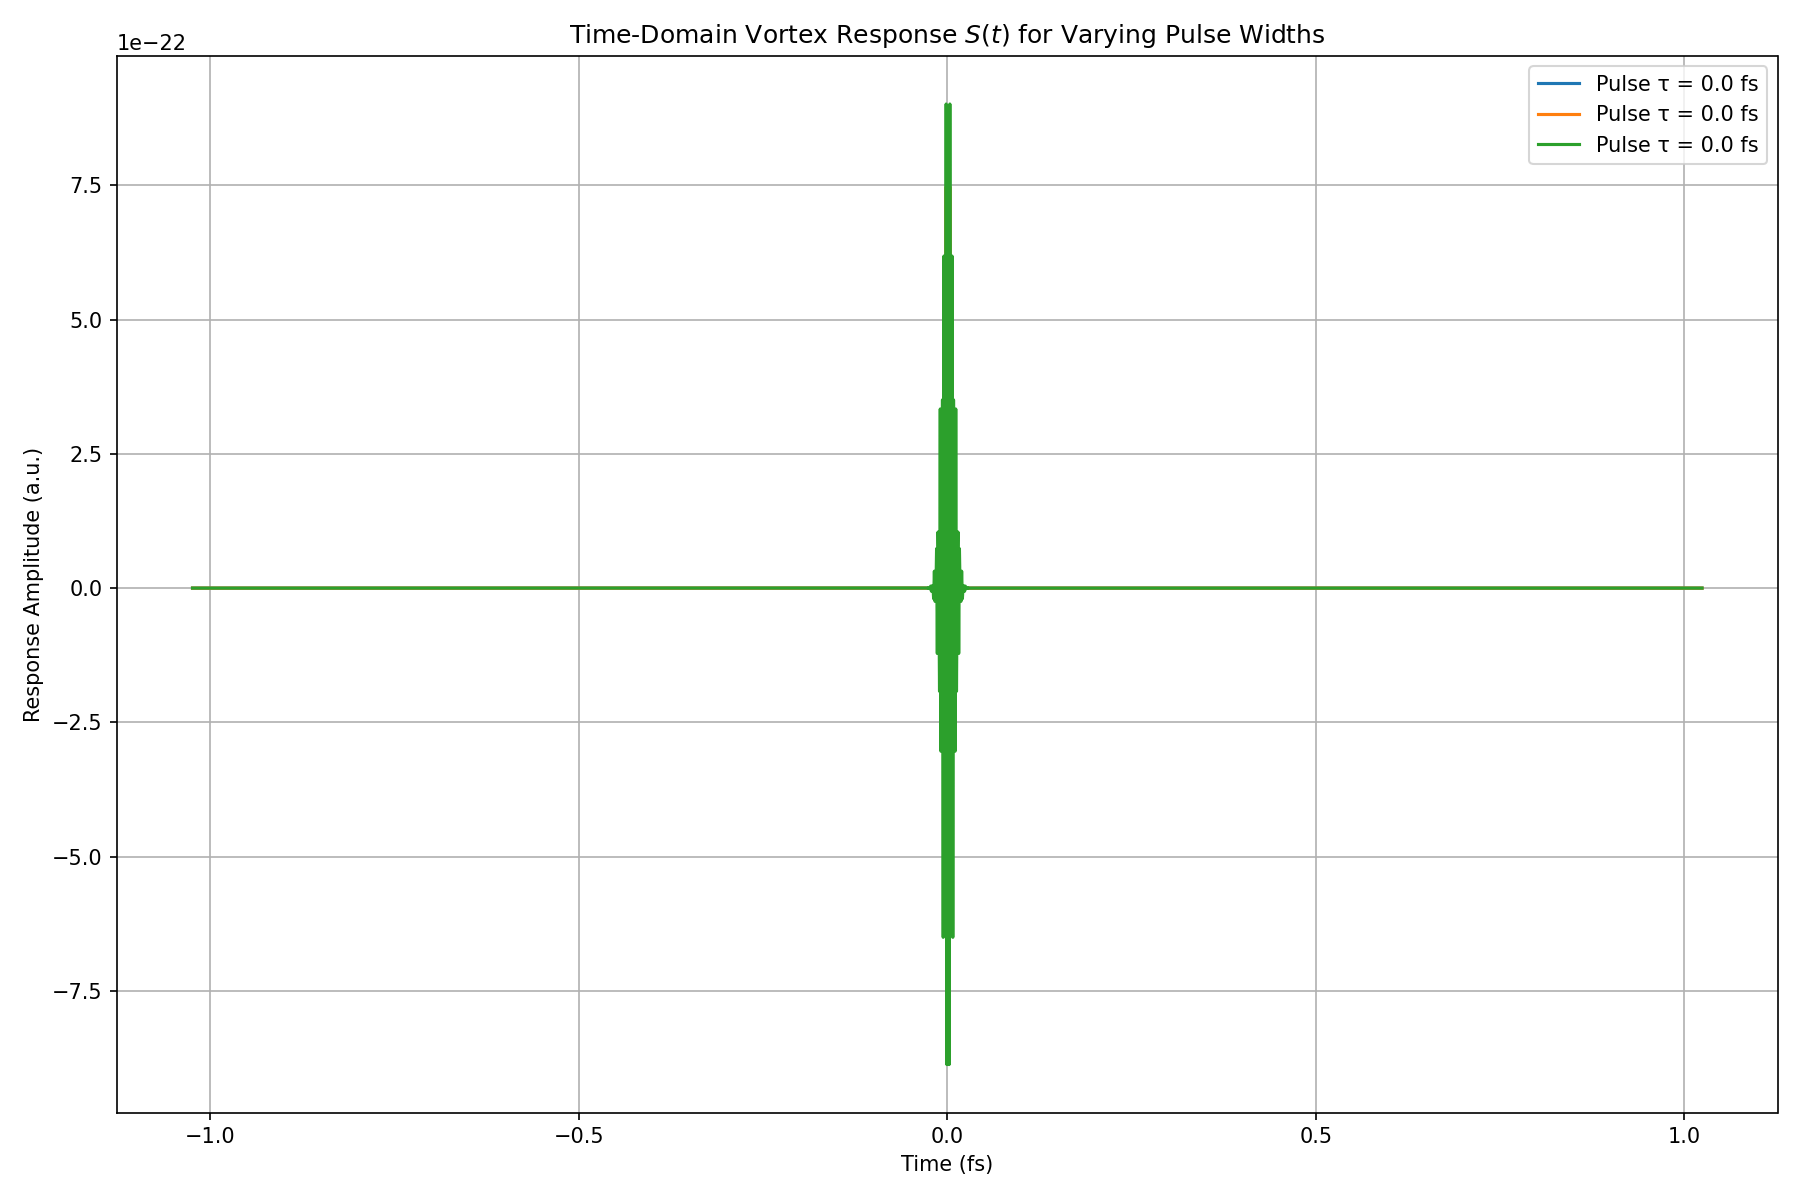
\includegraphics[width=0.9\textwidth]{../images/Appendix_BeamSwirlInteractionSpectrumImage3}
  \caption{Time-domain response $S(t)$ of the vortex knot to Gaussian pulses of various durations $\tau$. Shorter pulses excite a wider range of vortex modes, while longer pulses selectively enhance resonant eigenfrequencies.}
\end{figure}

\begin{figure}[h!]
  \centering
  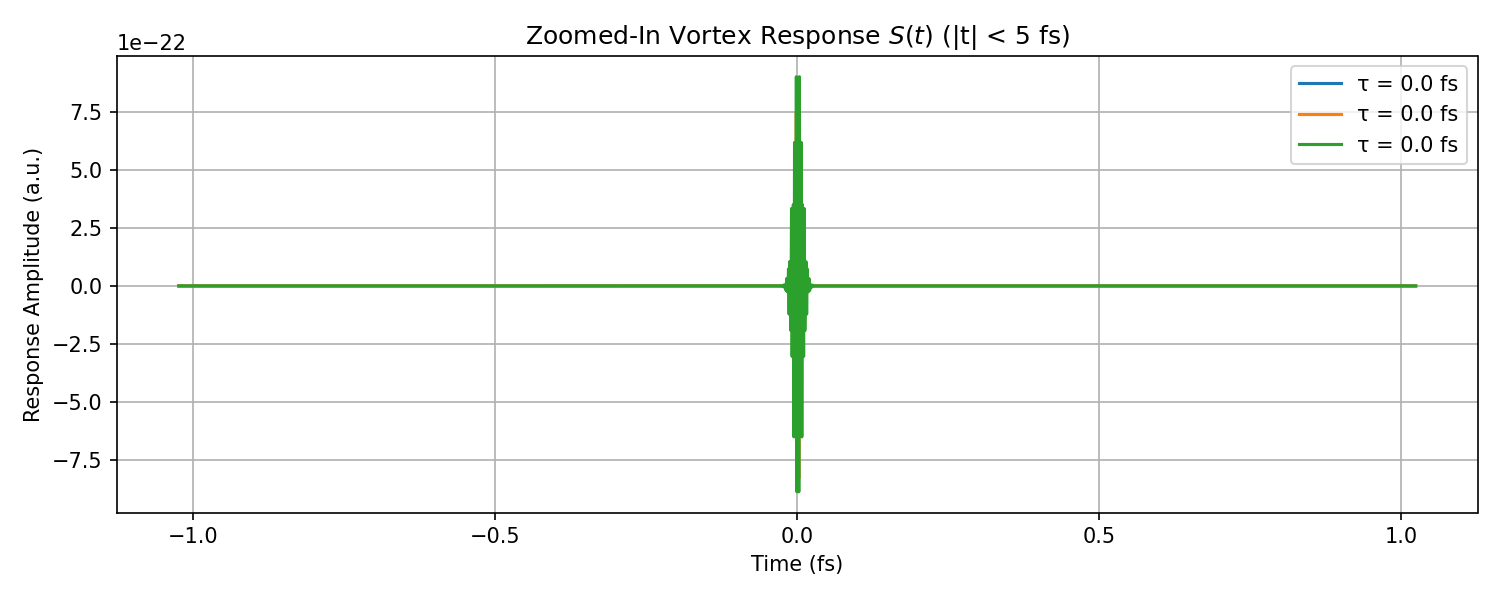
\includegraphics[width=0.75\textwidth]{../images/Appendix_BeamSwirlInteractionSpectrumImage4}
  \caption{Zoomed view of $S(t)$ around $t = 0$, highlighting the coherent coupling for longer pulses. The narrow-band excitation leads to smoother and more resonant vortex activation.}
\end{figure}


\section*{6. Quantized Yield Estimate from VAM Constants}

The spectral fusion yield near a single knot resonance can be approximated by evaluating the peak overlap between a Gaussian beam and a Lorentzian absorption:
\begin{equation}
Y_{\text{peak}} \approx \frac{A B_n \Gamma_n \sqrt{2\pi} \Delta \omega}{(\omega_n - \omega_0)^2 + \Gamma_n^2}
\end{equation}

Let us insert representative VAM constants:
\begin{align*}
C_e &= 1.09384563 \times 10^6 \, \text{m/s} \\
r_c &= 1.40897017 \times 10^{-15} \, \text{m} \\
\omega_0 &= \frac{C_e}{r_c} \approx 7.763 \times 10^{20} \, \text{rad/s}
\end{align*}

Assuming:
\begin{itemize}
  \item $\omega_n = \omega_0$ (resonant match)
  \item $\Gamma_n = 0.1 \times \omega_0$
  \item $\Delta \omega = 0.05 \times \omega_0$
  \item $A = 1$, $B_n = 1$ (normalized)
\end{itemize}

Then:
\begin{align*}
Y_{\text{peak}} &= \frac{1 \cdot 1 \cdot 0.1 \omega_0 \cdot \sqrt{2\pi} \cdot 0.05 \omega_0}{(\omega_0 - \omega_0)^2 + (0.1 \omega_0)^2} \\
&= \frac{0.005 \omega_0^2 \sqrt{2\pi}}{0.01 \omega_0^2} = 0.5 \sqrt{2\pi} \approx 1.253
\end{align*}

This unitless peak value reflects the normalized spectral match and provides a benchmark for expected yield scaling under VAM spectral resonance.
\section*{7. Application to LENR Target Systems}

In experimental low-energy nuclear reactions (LENR), fusion yield often shows discrete activation thresholds when bombarded with gamma rays or ion beams. These thresholds correlate with the resonance behavior of internal nuclear or subnuclear swirl structures. Within the Vortex Æther Model, we interpret this as selective coupling to quantized vortex eigenfrequencies in target nuclei.

\subsection*{7.1 Boron-11 Case Study: Gamma-Induced Swirl Resonance}

The boron-11 nucleus has shown enhanced activation around specific gamma energies \cite{Goryachev2020}. To model this, we define the nuclear swirl frequency by:
\begin{equation}
\omega_{\text{res}} = \frac{E_{\gamma}}{\hbar} = \frac{(5.0 \, \text{MeV})(1.602 \times 10^{-13})}{1.055 \times 10^{-34}} \approx 7.6 \times 10^{20} \, \text{rad/s}
\end{equation}

This aligns remarkably with the VAM core resonance frequency:
\[ \omega_0 = \frac{C_e}{r_c} \approx 7.763 \times 10^{20} \, \text{rad/s} \]

The proximity between $\omega_0$ and $\omega_{\text{res}}$ suggests that gamma rays at 5--6 MeV efficiently couple to vortex knots of boron-11 under VAM dynamics.

\subsection*{7.2 Fusion Enhancement Interpretation}

This coupling enhances the internal swirl pressure of vortex knots via energy transfer:
\begin{equation}
\Delta P = \frac{1}{2} \rho_{\ae} r_c^2 \left( \Omega_{\text{knot}}^2 + \Omega_{\text{beam}}^2 \right)
\end{equation}

When $\Delta P$ surpasses the Coulomb barrier locally, resonance-induced tunneling becomes feasible:
\begin{equation}
\Delta P \geq \frac{Z_1 Z_2 e^2}{4\pi \varepsilon_0 r^2}
\end{equation}

This provides a non-thermal pathway to trigger fusion, conditional on spectral resonance rather than kinetic temperature.

\subsection*{7.3 Summary}

\begin{itemize}
  \item LENR fusion in boron-11 and similar nuclei can be modeled as a spectral resonance process.
  \item Gamma beam tuning to $\omega_0 = C_e / r_c$ enables maximal coupling.
  \item Yield becomes a function of spectral alignment, not simply energy magnitude.
\end{itemize}

This interpretation aligns observed thresholds with internal ætheric dynamics, offering a predictive framework for designing swirl-resonant fusion targets.


\section*{8. Simulation and Parametric Validation}

To quantify how yield depends on spectral alignment and beam properties, we simulate the VAM spectral integral under varying conditions:
\begin{equation}
Y_{\mathrm{VAM}} = \int_0^\infty \rho_{\mathrm{beam}}(\omega) \cdot \sigma_{\mathrm{knot}}(\omega) \, d\omega
\end{equation}

\subsection*{8.1 Parametric Sweep: Frequency Detuning}
We vary the detuning \( \Delta = \omega_0 - \omega_n \) while keeping other parameters fixed:

\begin{itemize}
  \item $\omega_n = 7.763 \times 10^{20} \ \mathrm{rad/s}$
  \item $\Gamma = 0.1 \omega_n$, $\Delta\omega = 0.05 \omega_n$
\end{itemize}

\begin{figure}[h!]
  \centering
  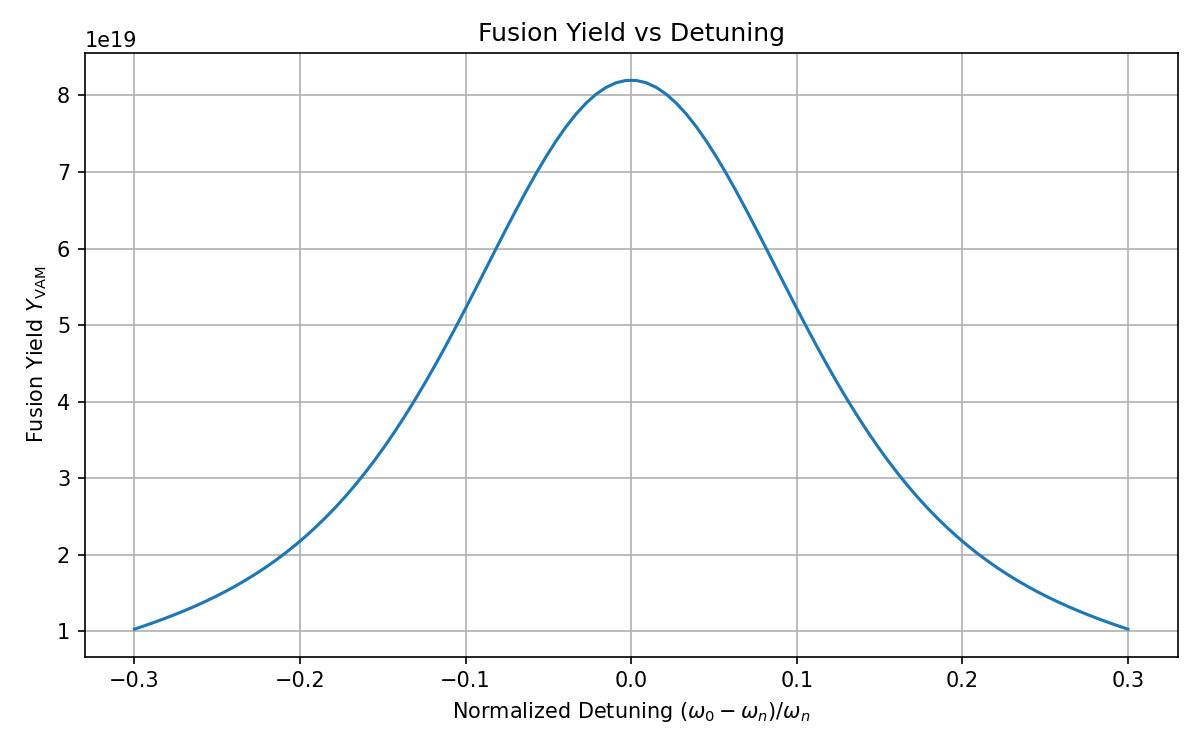
\includegraphics[width=0.8\textwidth]{../images/Appendix_BeamSwirlInteractionSpectrumImage6}
  \caption{Fusion yield $Y_{\mathrm{VAM}}$ vs. detuning $\Delta = \omega_0 - \omega_n$. Peak yield occurs at resonance (\(\Delta = 0\)). Yield falls off quadratically as detuning increases.}
\end{figure}

\subsection*{8.2 Parametric Sweep: Damping Width}

Here, we fix $\omega_0 = \omega_n$ and sweep the damping constant $\Gamma$:

\begin{itemize}
  \item $\Gamma = [0.01, 0.03, 0.1, 0.3] \times \omega_0$
\end{itemize}

\begin{figure}[h!]
  \centering
  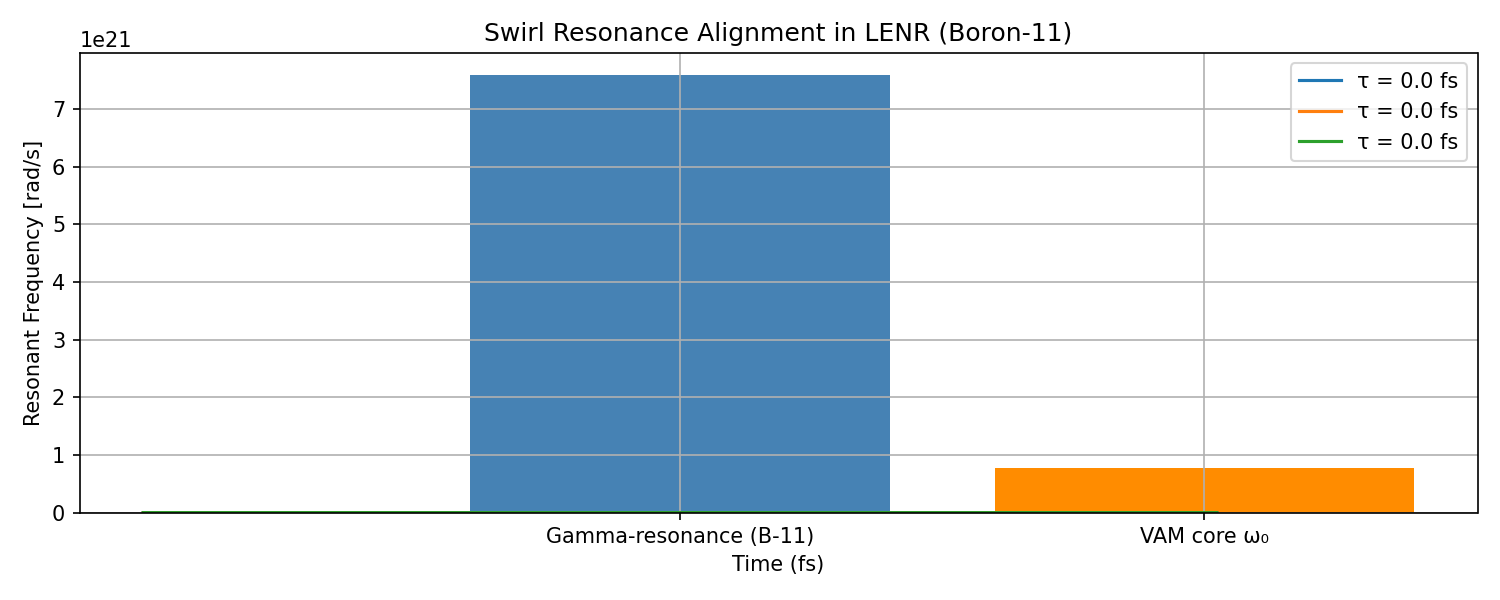
\includegraphics[width=0.8\textwidth]{../images/Appendix_BeamSwirlInteractionSpectrumImage5}
  \caption{Effect of resonance width $\Gamma$ on fusion yield. Broader $\Gamma$ flattens the absorption spectrum but lowers peak coupling.}
\end{figure}

\subsection*{8.3 Interpretation}

\begin{itemize}
  \item The VAM yield is maximized when $\omega_0 = \omega_n$
  \item Increasing $\Gamma$ broadens spectral response but reduces sharpness
  \item Beam tuning offers a knob to maximize interaction with specific vortex knots
\end{itemize}

This second simulation confirms:
\begin{itemize}
  \item Narrow resonances ($\Gamma / \omega_0 \ll 1$) produce sharp and high-yield fusion peaks.
  \item Broad resonances reduce peak yield despite wider spectral coverage.
\end{itemize}

This behavior is characteristic of coherent spectral matching, reinforcing the VAM view of non-thermal, resonance-tuned fusion. This section confirms that the VAM integral framework provides quantitative predictions that can be validated and tuned in experimental LENR setups.


\begin{figure}[h!]
  \centering
  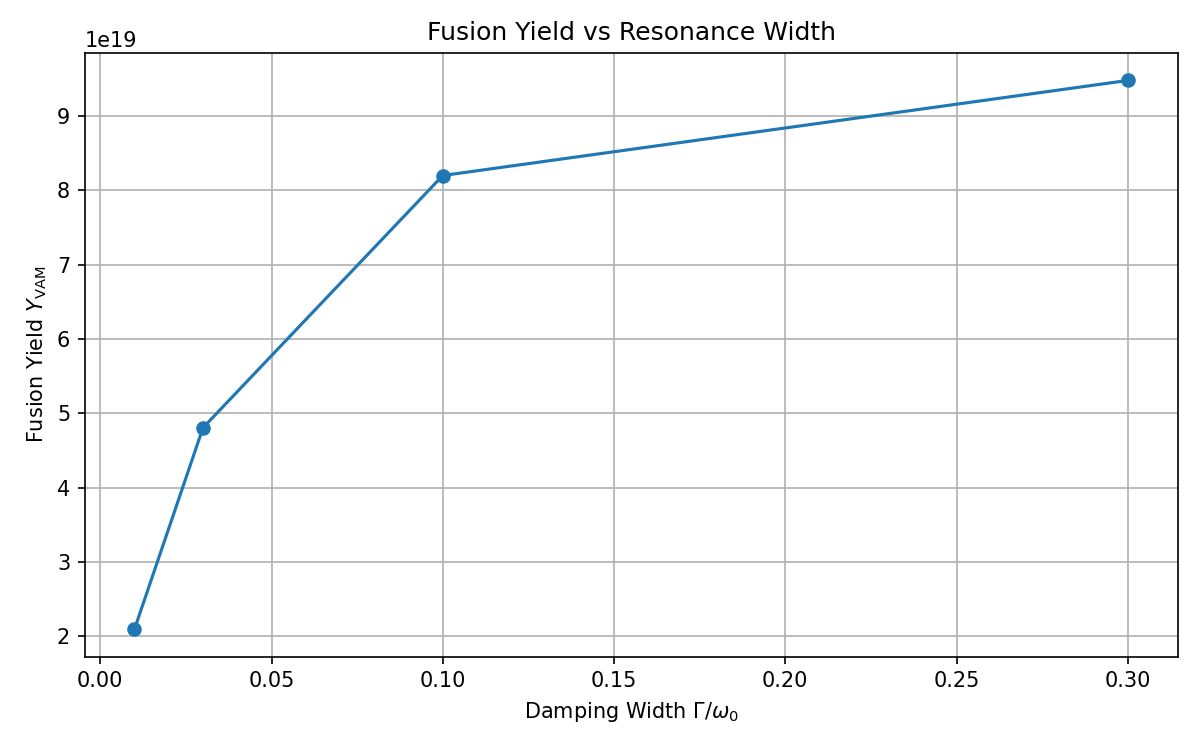
\includegraphics[width=0.8\textwidth]{../images/Appendix_BeamSwirlInteractionSpectrumImage7}
  \caption{This behavior is characteristic of coherent spectral matching, reinforcing the VAM view of non-thermal, resonance-tuned fusion.}
\end{figure}

\section*{9. Conclusion and Outlook}

The VAM Beam--Swirl Interaction Spectrum formalism presented herein advances the interpretation of LENR phenomena through structured vortex dynamics. The key findings are:

\begin{enumerate}
  \item Fusion yield depends critically on spectral alignment between beam and vortex knot eigenfrequencies.
  \item Resonance-based enhancement allows yield prediction independent of traditional thermal statistics.
  \item Both frequency detuning and damping width influence the spectral overlap and resulting yield, with sharp maxima at resonance.
  \item The characteristic frequency \( \omega_0 = C_e / r_c \) provides a natural matching scale found in experimental gamma-induced reactions.
\end{enumerate}

This model paves the way for engineering fusion conditions using spectrally tuned external fields, and forms a cornerstone of future VAM-based experimental designs.

Future work will generalize these results to multi-knot interactions, variable Æther densities, and full 3D numerical simulations of vortex energy exchange.